%!Mode:: "TeX:UTF-8"
\documentclass[a4paper,11pt,UTF8]{ctexart}

\usepackage{indentfirst} %缩进
\usepackage{xeCJK}    %使用系统字体
\usepackage{fancyhdr} %自定义页眉页脚
\pagestyle{empty}                   %不设置页眉页脚
\usepackage{amsmath, amsthm, amssymb, amsfonts} %数学公式
\usepackage[a4paper,left=3cm,right=3cm,top=3cm,bottom=3cm]{geometry}
%\usepackage[tmargin=1in,bmargin=1in,lmargin=1.25in,rmargin=1.25in]{geometry}.
\usepackage{booktabs} %插入表格
\usepackage[section]{placeins} %避免浮动
\usepackage{listings} %插入代码
\usepackage{ctex}     %中文宏包
\usepackage[svgnames, table]{xcolor} %彩色表格
\usepackage{algorithm}          %伪代码
\usepackage{algorithmicx}
\usepackage{algpseudocode}
\usepackage{algorithm,algpseudocode,float}
\usepackage{lipsum}
\usepackage{enumitem}           %调整列举环境
\usepackage{url}
\usepackage{fontspec,xunicode}
\defaultfontfeatures{Mapping=tex-text} %如果没有它,会有一些 tex 特殊字符无法正常使用,比如连字符。

\usepackage{graphicx}
\graphicspath{{imgs/}}

%%%%%%%%%%%%%%%%%%%%%%%%%%%%%%%%%%%%%%%%%%%%%%%%%%%%%%%%%%%%%%%%
% 缩进及行间距
%%%%%%%%%%%%%%%%%%%%%%%%%%%%%%%%%%%%%%%%%%%%%%%%%%%%%%%%%%%%%%%%
\setlength{\parindent}{22pt} %重新定义缩进长度
\setlength{\baselineskip}{20pt}  %定义行间距
%\renewcommand{\baselinestretch}{1.1} %定义行间距
%%%%%%%%%%%%%%%%%%%%%%%%%%%%%%%%%%%%%%%%%%%%%%%%%%%%%%%%%%%%%%%%
% 数学符号
%%%%%%%%%%%%%%%%%%%%%%%%%%%%%%%%%%%%%%%%%%%%%%%%%%%%%%%%%%%%%%%%
\newcommand\pd{\partial}
\newcommand\dd{\thinspace\mathrm{d}}
\newcommand\pdone[2]{\frac{\pd #1}{\pd #2}}
\newcommand\pdtwo[2]{\frac{\pd^2 #1}{\pd #2 ^2}}
\newcommand\ddone[2]{\frac{\dd #1}{\dd #2}}
\newcommand\ddtwo[2]{\frac{\dd^2 #1}{\dd #2 ^2}}
%%%%%%%%%%%%%%%%%%%%%%%%%%%%%%%%%%%%%%%%%%%%%%%%%%%%%%%%%%%%%%%%
% 列表设置
%%%%%%%%%%%%%%%%%%%%%%%%%%%%%%%%%%%%%%%%%%%%%%%%%%%%%%%%%%%%%%%%
\setenumerate{fullwidth,itemindent=\parindent,listparindent=\parindent,itemsep=0ex,partopsep=0pt,parsep=0ex}
\setenumerate[2]{label=\alph*),leftmargin=1.5em}  %二级item设置
\setitemize{itemindent=38pt,leftmargin=0pt,itemsep=-0.4ex,listparindent=26pt,partopsep=0pt,parsep=0.5ex,topsep=-0.25ex}
\setdescription{itemindent=38pt,leftmargin=0pt,itemsep=-0.4ex,listparindent=26pt,partopsep=0pt,parsep=0.5ex,topsep=-0.25ex}

%%%%%%%%%%%%%%%%%%%%%%%%%%%%%%%%%%%%%%%%%%%%%%%%%%%%%%%%%%%%%%%%
% 图的标题行间距设置
%%%%%%%%%%%%%%%%%%%%%%%%%%%%%%%%%%%%%%%%%%%%%%%%%%%%%%%%%%%%%%%%
\newcommand{\bottomcaption}{%
\setlength{\abovecaptionskip}{6pt}%
\setlength{\belowcaptionskip}{6pt}%
\caption}


%%%%%%%%%%%%%%%%%%%%%%%%%%%%%%%%%%%%%%%%%%%%%%%%%%%%%%%%%%%%%%%%
% 字体定义
%%%%%%%%%%%%%%%%%%%%%%%%%%%%%%%%%%%%%%%%%%%%%%%%%%%%%%%%%%%%%%%%
\setmainfont{Times New Roman}  %默认英文字体.serif是有衬线字体sans serif无衬线字体
\setmonofont{Consolas}
\setCJKmainfont[ItalicFont={楷体}, BoldFont={黑体}]{宋体}%衬线字体 缺省中文字体为
\setCJKsansfont{黑体}
\punctstyle{hangmobanjiao}
%-----------------------xeCJK下设置中文字体------------------------------%
\setCJKfamilyfont{song}{SimSun}                             %宋体 song
\newcommand{\song}{\CJKfamily{song}}
\setCJKfamilyfont{fs}{FangSong}                      %仿宋  fs
\newcommand{\fs}{\CJKfamily{fs}}
\setCJKfamilyfont{ktgb}{KaiTi}                      %楷体2312 ktgb
\newcommand{\ktgb}{\CJKfamily{ktgb}}
\setCJKfamilyfont{yh}{Microsoft YaHei}                    %微软雅黑 yh
\newcommand{\yh}{\CJKfamily{yh}}
\setCJKfamilyfont{hei}{SimHei}                              %黑体  hei
\newcommand{\hei}{\CJKfamily{hei}}
\setCJKfamilyfont{hwxk}{STXingkai}                                %华文行楷  hwxk
\newcommand{\hwxk}{\CJKfamily{hwxk}}
%------------------------------设置字体大小------------------------%
\newcommand{\shiyanbaogao}{\fontsize{36pt}{\baselineskip}\selectfont}
\newcommand{\chuhao}{\fontsize{42pt}{\baselineskip}\selectfont}     %初号
\newcommand{\xiaochuhao}{\fontsize{36pt}{\baselineskip}\selectfont} %小初号
\newcommand{\yihao}{\fontsize{28pt}{\baselineskip}\selectfont}      %一号
\newcommand{\erhao}{\fontsize{21pt}{\baselineskip}\selectfont}      %二号
\newcommand{\xiaoerhao}{\fontsize{18pt}{\baselineskip}\selectfont}  %小二号
\newcommand{\sanhao}{\fontsize{15.75pt}{\baselineskip}\selectfont}  %三号
\newcommand{\sihao}{\fontsize{14pt}{\baselineskip}\selectfont}       %四号
\newcommand{\xiaosihao}{\fontsize{12pt}{\baselineskip}\selectfont}  %小四号
\newcommand{\wuhao}{\fontsize{10.5pt}{\baselineskip}\selectfont}    %五号
\newcommand{\xiaowuhao}{\fontsize{9pt}{\baselineskip}\selectfont}   %小五号
\newcommand{\liuhao}{\fontsize{7.875pt}{\baselineskip}\selectfont}  %六号
\newcommand{\qihao}{\fontsize{5.25pt}{\baselineskip}\selectfont}    %七号

%%%%%%%%%%%%%%%%%%%%%%%%%%%%%%%%%%%%%%%%%%%%%%%%%%%%%%%%%%%%%%%%
% 图题字体大小相同
%%%%%%%%%%%%%%%%%%%%%%%%%%%%%%%%%%%%%%%%%%%%%%%%%%%%%%%%%%%%%%%%
\usepackage{caption}
\captionsetup{font={footnotesize}}   % footnotesize = 9pt
\captionsetup[lstlisting]{font={footnotesize}}

%%%%%%%%%%%%%%%%%%%%%%%%%%%%%%%%%%%%%%%%%%%%%%%%%%%%%%%%%%%%%%%%
% 重定义枚举编号为 1),2)...
%%%%%%%%%%%%%%%%%%%%%%%%%%%%%%%%%%%%%%%%%%%%%%%%%%%%%%%%%%%%%%%%
\renewcommand{\labelenumi}{\theenumi)}

%%%%%%%%%%%%%%%%%%%%%%%%%%%%%%%%%%%%%%%%%%%%%%%%%%%%%%%%%%%%%%%%
% 标题名称中文化
%%%%%%%%%%%%%%%%%%%%%%%%%%%%%%%%%%%%%%%%%%%%%%%%%%%%%%%%%%%%%%%%
\renewcommand\figurename{\hei 图}
\renewcommand\tablename{\hei 表}
\renewcommand\lstlistingname{\hei 代码}
\renewcommand{\algorithmicrequire}{\textbf{输入:}}
\renewcommand{\algorithmicensure}{\textbf{输出:}}
\newtheorem{define}{定义}

%%%%%%%%%%%%%%%%%%%%%%%%%%%%%%%%%%%%%%%%%%%%%%%%%%%%%%%%%%%%%%%%
% 代码设置
%%%%%%%%%%%%%%%%%%%%%%%%%%%%%%%%%%%%%%%%%%%%%%%%%%%%%%%%%%%%%%%%
\lstset{
 columns=fixed,
 numbers=left,                                        % 在左侧显示行号
 numberstyle=\tiny\color{gray},                       % 设定行号格式
 frame=single,                                        % 单线背景边框
 breaklines=true,                                     % 设定LaTeX对过长的代码行进行自动换行
 keywordstyle=\color[RGB]{40,40,255},                 % 设定关键字颜色
 numberstyle=\footnotesize\color{darkgray},
 commentstyle=\it\color[RGB]{0,96,96},                % 设置代码注释的格式
 stringstyle=\rmfamily\slshape\color[RGB]{128,0,0},   % 设置字符串格式
 showstringspaces=false,                              % 不显示字符串中的空格
 language=java,                                        % 设置语言
 basicstyle=\linespread{1.0}\xiaowuhao\ttfamily,                      % 字体字号
 %lineskip=10pt,
 %baselinestretch=1,
}

%%%%%%%%%%%%%%%%%%%%%%%%%%%%%%%%%%%%%%%%%%%%%%%%%%%%%%%%%%%%%%%%
% 伪代码分页
%%%%%%%%%%%%%%%%%%%%%%%%%%%%%%%%%%%%%%%%%%%%%%%%%%%%%%%%%%%%%%%%
\makeatletter
\renewcommand{\ALG@name}{算法}
\newenvironment{breakablealgorithm}
  {% \begin{breakablealgorithm}
   \begin{center}
     \refstepcounter{algorithm}% New algorithm
     \hrule height.8pt depth0pt \kern2pt% \@fs@pre for \@fs@ruled
     \renewcommand{\caption}[2][\relax]{% Make a new \caption
       {\raggedright\textbf{\ALG@name~\thealgorithm} ##2\par}%
       \ifx\relax##1\relax % #1 is \relax
         \addcontentsline{loa}{algorithm}{\protect\numberline{\thealgorithm}##2}%
       \else % #1 is not \relax
         \addcontentsline{loa}{algorithm}{\protect\numberline{\thealgorithm}##1}%
       \fi
       \kern2pt\hrule\kern2pt
     }
  }{% \end{breakablealgorithm}
     \kern2pt\hrule\relax% \@fs@post for \@fs@ruled
   \end{center}
  }
\makeatother

% =============================================
% Part 1 Edit the info
% =============================================

\newcommand{\major}{物理学院}
\newcommand{\name}{黄阅迅,李秋阳}
\newcommand{\stuid}{PB18020631,PB18020567}
\newcommand{\group}{20}
\newcommand{\newdate}{\today}


\newcommand{\course}{电子线路实验(1)}
\newcommand{\newtitle}{一阶电路的研究}

% =============================================
% Part 1 Main document
% =============================================
\begin{document}
\thispagestyle{empty}
\begin{figure}[h]
  \begin{minipage}{0.6\linewidth}
    \centerline{
\includegraphics[width=\linewidth]{logo.png}}
  \end{minipage}
  \hfill
  \begin{minipage}{.4\linewidth}
    \raggedleft
    \begin{tabular*}{.8\linewidth}{ll}
      学院: & \underline\major   \\
      姓名: & \underline\name    \\
      学号: & \underline\stuid   \\
      组号:  & \underline\group   \\
      日期: & \underline\newdate \\
    \end{tabular*}
  \end{minipage}
\end{figure}

\begin{table}[!htbp]
  \centering
  \begin{tabular*}{\linewidth}{llllll}
    课程名称:  \underline\course   \qquad\qquad 实验题目:  \underline\newtitle  
  \end{tabular*}
\end{table}

% =============================================
% Part 2 Main document
% =============================================

\section{实验目的}
参见预习报告。
\section{实验原理}
参见预习报告。
\section{实验内容与步骤}
\subsection{实验内容}
\begin{itemize}
  \item 利用示波器测量一阶电路中零状态响应和零输入响应的时间常数;
  \item 利用RC电路搭建微分和积分运算电路,并测量波形;
  \item 搭建脉冲分压电路,并测量波形。
\end{itemize}
	
\subsection{实验步骤}
  \subsubsection{RC一阶电路零输入和零状态响应}
  \begin{enumerate}
    \item 搭建如图 \ref{fig:react}所示的电路,调节电路参数为$R_1=200\Omega,R=1k\Omega,C=0.1\mu F$。
    \item 调整整流后$U_p=5V$,观察阶跃响应和零输入响应。
    \item 定量画出波形图并分析。
  \end{enumerate}
  \begin{figure}[htbp]
    \centering
    \fbox{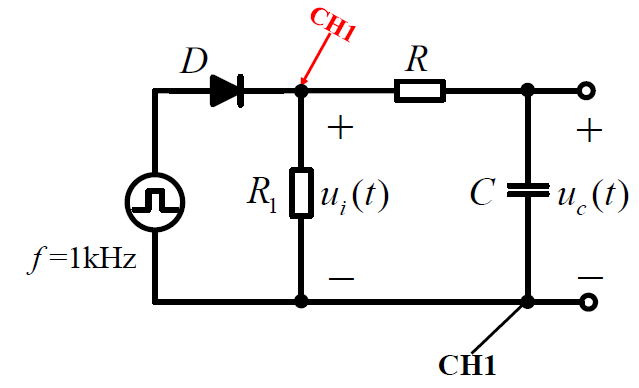
\includegraphics[width=0.5\linewidth]{react.PNG}}
    \caption{一阶电路零输入和零状态响应测量图}
    \label{fig:react}
    \end{figure}
  \subsection{RC积分电路}
  \begin{enumerate}
    \item 搭建如图 \ref{fig:RCInt}所示的电路,调节电路参数为$R_1=200\Omega,R=10k\Omega,C=1\mu F$。
    \item 画出波形图,并测出有关的波形参数。
  \end{enumerate}
  \begin{figure}[htbp]
    \centering
    \fbox{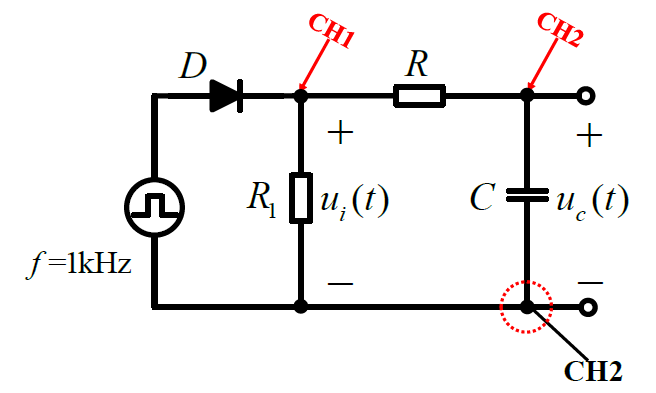
\includegraphics[width=0.5\linewidth]{RCInt.PNG}}
    \caption{RC积分电路示意图}
    \label{fig:RCInt}
    \end{figure}
  \subsection{RC微分电路}
  \begin{enumerate}
    \item 搭建如图 \ref{fig:RCDev}所示的电路,调节电路参数为$R_1=200\Omega,R=1k\Omega,C=0.05\mu F$。
    \item 画出波形图,并测出有关的波形参数。
  \end{enumerate}
  \begin{figure}[htbp]
    \centering
    \fbox{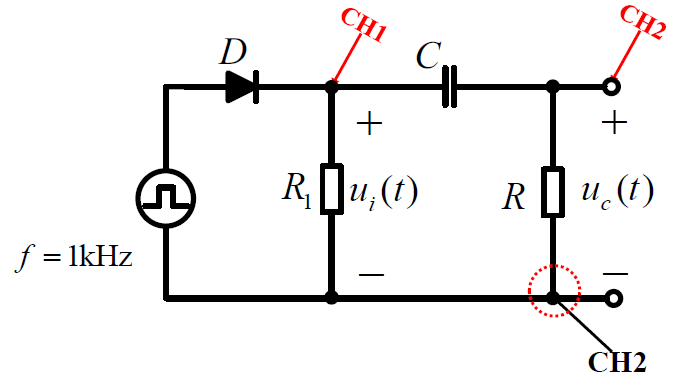
\includegraphics[width=0.5\linewidth]{RCDev.PNG}}
    \caption{RC微分电路示意图}
    \label{fig:RCDev}
    \end{figure}
  \subsection{脉冲分压电路}
  \begin{enumerate}
    \item 搭建如图 \ref{fig:bleeder}所示的电路,调节电路参数为$R_1=20k\Omega,R_2=10k\Omega,C_1=0.005\mu F,C_2=0.01\mu F$。
    \item 测量输入和输出波形,画出波形图,并测出有关的波形参数。
  \end{enumerate}
  \begin{figure}[htbp]
    \centering
    \fbox{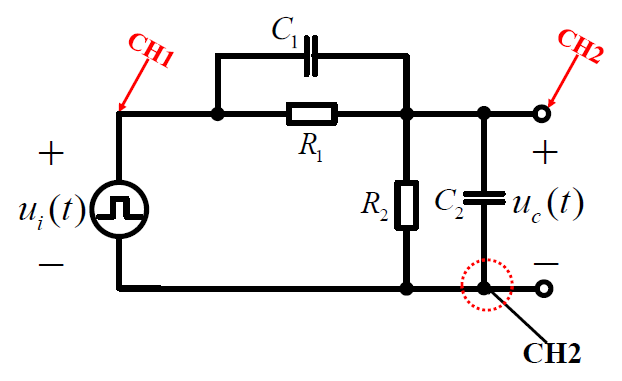
\includegraphics[width=0.5\linewidth]{bleeder.PNG}}
    \caption{脉冲分压电路示意图}
    \label{fig:bleeder}
    \end{figure}

\section{实验数据处理与分析}
\subsection{RC一阶电路零输入和零状态响应}
实验所测得波形图如附图一所示。所测得零状态与零输入响应的时间常数分别为
\begin{equation}
  \tau_1=0.109ms;~\tau_2=0.116ms;
\label{eqa:timeConstant}
\end{equation}
可见相差不大,而理论上给出时间常数为
\begin{equation}
  \tau_{theory}=RC=0.1ms
\end{equation}
对比可见与理论值吻合得较好。
\subsection{误差分析1}
对零状态和零输入的均方根相对误差为
\begin{equation}
  RE_1=\left|\frac{0.109-0.1}{0.1}\right|\times100\%=9\%;\;
  RE_2=\left|\frac{0.116-0.1}{0.1}\right|\times100\%=16\%;
\end{equation}
可见百分比误差略大,而在零输入响应的误差与理论值相差更大。这应该是测量的误差造成的,示波器的最小分度值为$0.2V$,因此在测量时间常数对应的电压点时
无法与格线对其,有较大的读数误差。同时,零输入状态下曲线为凹函数,因此判断的误差更大。
\subsection{RC积分电路}
RC积分电路测得波形图如附图一所示。则从图中可根据积分电路电压关系求出被积电压
\begin{equation}
  P(t)=\tau \frac{d u_{c}}{dt}=1\mu F\times10k\Omega\times\frac{2.645V-2.415V}{0.5ms}\approx5V
\end{equation}
波形图在稳定时上下端峰值几乎维持不变。
\subsection{误差分析2}
可见在当前有效数字下,计算预测结果与实际结果$5V$完全吻合。说明在当前精度下,与理论吻合得相当好。但实际上考虑多一位有效数字时,$\Delta V=0.4V$。实验误差主要来自示波器读数,但电容箱的电容可能并不准确,导致理论值可能出现
一定偏差。
\subsection{RC微分电路}
实验测得波形图中的上峰值为$U_{p+}=4.76V$,下峰值为$U_{p-}=-4.04V$。波形在峰后$0.2ms$后降至$0V$并保持稳定。波形图如附图三所示。理论给出
\begin{equation}
  u_R(0+)\rightarrow+\infty V;\; u_R(t)=0V,~t\in(0,0.5)
\end{equation}
\subsection{误差分析3}
可见理论预测与实际相差较大,但也有一定的吻合段。这是因为函数信号发生器产生方波,实际上有一定的上升时间,因此斜率实际上不会达到狄拉克函数预测的正负无穷。
同时示波器的时间取样有一定的区间,电压的读取范围也有一定区间,因此读出的上下峰值是较为不准的。基本波形图上暗示了电压可能趋向正无穷的趋势。因此可以认为在实验误差允许范围内,结果可以接受。
\subsection{脉冲分压电路}
实验测得的波形图如附图四所示。测得的输出稳定电压值为$u_o=1.00V$。理论计算所得为
\begin{equation}
  u_{oTheory}=\frac{R_2}{R_1+R_2}\times u_i=1V
\end{equation}
可见理论与实验测得值较为吻合。但实际图像上,输出电压在上峰值时表现出先下降后稳定的图像,而保持较好的稳定时需要将电容$C_2$校准至$0.014\mu F$,否则出现过补偿现象。
\subsection{误差分析4}
最终稳定值与理论符合得相当好,但实际波形有差异。这可能由两个原因造成,一个是电容箱的电容值可能不准,第二是电阻箱的电阻可能本身带有一定得容性,这也造成了如此得实验现象。实际观察输入电压,也有细微的先下降后平稳的现象,这应该是
电阻带容性造成的。
\section{实验总结}
在本次实验中,我们利用示波器搭建与测量了RC一阶电路的响应电路、微分和积分电路以及脉冲分压电路
虽然有一定的误差,但在实验设计允许范围内,和理论吻合得较好,成果较为令人满意。通过这次实验也学习到了
一阶电路的一些特性,熟悉了时间常数有关的概念,锻炼了实验能力和误差分析能力。
\newpage
\section{实验思考题}
\subsection{本次实验电路中,电阻$R_1$在电路中起何作用?}
\textbf{答:}起负载作用。因为在实验中,函数信号发生器给出的信号特性是不准确的,需要用示波器测量经过二极管后的信号特性。而函数信号发生器存在内阻,所以开路和带负载时测量的结果也是不一样的。所以要在等效电源(信号函数发生器与二极管的串联)两端接一个负载,这样才能比较准确地测量出等效电源输出信号的特性。
\subsection{本次实验中,能用毫伏表测量电阻$R_1$两端的矩形波电压么,为什么?}
\textbf{答:}不能。万用表毫伏表可能是直流电压档或者交流电压档。如果用直流电压档,那么因为电压值一直在变化,而且频率对于直流档来说太大,因此无法测准;如果用交流电压档,那么万用表给出的是正弦交流电的有效值,但是$R_1$两端是矩形电压,因此也无法测准。
\subsection{根据本次实验说明RC电路分别用作积分电路和微分电路必须具备的条件?}
\textbf{答:}用作积分电路的条件:$t_p\ll \tau=RC$,也即电源电压变化时间远小于时间常数。用作积分电路的条件:$t_p\gg \tau=RC$,也即电源电压变化时间远大于时间常数。
\subsection{脉冲分压器电路中,有两个贮能元件电容$C_1$和$C_2$,为何是一阶电路?}
\textbf{答:}二阶电路的真正定义是:电压/电流满足的关系式是二阶常微分方程。这里虽然有两个电容,但由于电容满足的关系式为:$i_c=C\ddone{u_c}{t}$,所以电路方程最后一定还是一阶常微分方程,所以电路还是一阶电路。
\end{document}
